\documentclass[12pt, a4paper]{article}
\usepackage{graphicx} % Required for inserting images

\title{Thesis}
\author{L.Y. Kogelheide}

%indent first lines
\usepackage{indentfirst}
\setlength{\parindent}{15pt}

%enhance math typesetting
\usepackage{amsmath}

\usepackage{multirow}

\usepackage{graphicx}

\usepackage{pdflscape}

\usepackage[style = authoryear,
    citestyle = authoryear, 
    giveinits = true
    sorting = nyt,
    sortcites = true,
    autopunct = true,
    babel = hyphen,
    hyperref = true,
    abbreviate = false,
    backref = false,
    dashed = false,
    maxcitenames = 2, % the maximum number of authors displayed in citations. 
    %maxnames = 99, % sets both maxbibnames and maxcitenames. 
    %Default value is 3
    maxbibnames = 99, % the maximum number of authors displayed in bibliography.
    %apamaxprtauth=999, % the maximum number of authors displayed in bibliography in apa
    uniquename = false,
    uniquelist = false,
    backend = biber]{biblatex}

\addbibresource{references.bib} 

\usepackage{setspace}
\doublespacing

\begin{document}

    \begin{center}

        \Large
        \textbf{Comparing machine learning and statistical models in capture-recapture estimators: a simulation study on bias and precision}
        \\
        \vspace{1cm}
        Research Report

        \vspace{1.5cm}
        \Large
        \textbf{Luca Y. Kogelheide (8159556)}

        \vspace{0.5cm}
        \large
        Supervisors: Dr. Joep Burger (CBS) and Dr. Jonas Klingwort (CBS)

        \vspace{1.5cm}
        Methodology and Statistics for the Behavioural, Biomedical and Social Sciences - Utrecht University

        \vspace{2cm}
        Date: 22.12.2024 \\
        Word count: 2498

        \thispagestyle{empty}

        \newpage
    
    \end{center}

\newpage

\setcounter{page}{1}

\section{Introduction}
\noindent The primary objective of national statistical institutes is to produce high-quality statistics that inform the public and guide policymakers \parencite{Eurostat}. Traditionally, such statistics are generated using probability surveys. However, in recent decades, several challenges associated with survey-based data collection have emerged, including declining response rates \parencite{de2018international, Meyer2015} and an increased response burden \parencite{richardson1996nonresponse, hu2017nonresponse}. These issues arise particularly in diary surveys, which are time-intensive and impose a substantial response burden on respondents. \par

As a result, participants may report inaccurately or do not respond at all, potentially resulting in significant underreporting \parencite{ashley2009underreporting, schmidt2014consumers}. Within the Total Survey Error Framework \parencite{biemer2010total}, such shortcomings are understood as both measurement error and nonresponse error, respectively, leading to biased estimates if not adequately addressed. While nonresponse error can often be mitigated through statistical weighting techniques, addressing measurement error remains challenging due to the difficulty of validating the amount. Typically, a second independent data source is needed to quantify the measurement error before it can be corrected. \par

One potential approach to quantifying measurement error is to link survey data to a second data source, thereby combining multiple data sources \parencite{lohr2017datasources}. \textcite{klingwort2019CRC} proposed using capture-recapture (CRC) techniques to quantify measurement error by linking survey data with sensor data as a secondary data source. Although weighting the survey estimates can account for selective nonresponse, the CRC estimators offer the additional advantage of correcting for measurement error. By comparing the counts and characteristics of the units in both data sources, CRC estimators estimate the portion of the population that is misclassified or unobserved in either data source, thus correcting for measurement errors such as underreporting. The difference between the basic survey estimate and the CRC estimate is the estimated amount of measurement error in the survey. An in-depth study comparing multi-source model-based CRC estimates with design-based survey estimates identified underreporting, likely due to the high (perceived) response burden, as the cause for the difference between survey and CRC estimates \parencite{klingwort2021transition}. 

\section{Research Background}
\noindent Recent advances in machine learning (ML) have expanded its applications within the field of capture-recapture methodologies. For example, in ecological research, ML is predominantly applied to automate labor-intensive and time-consuming tasks such as labeling images produced by camera traps \parencite{whytock2021robust, green2020spatially} or identifying animals through data from bioacoustic sensors \parencite{wang2024statistical}. However, one topic that has received limited attention so far is the application of ML algorithms in the capture-recapture estimation process. Model-based CRC estimators use additional information to improve the accuracy of the estimate. Usually, this is done by applying regression models to map these covariates to the target variable. Since ML algorithms are highly flexible in capturing complex, non-linear relationships \parencite{boulesteix2014machine}, they might provide more accurate predictions than statistical models and thus provide better estimates. \par

In a recent study, \textcite{walraad2024MLCRC} explored the application of gradient boosting algorithms, specifically XGBoost, in the context of model-based CRC estimators. By applying both XGBoost and generalized linear models (GLM) to map auxiliary variables to the target variable, the study demonstrated that ML-based approaches outperform statistical models in terms of predictive accuracy. However, improvements in prediction performance had little impact on the resulting CRC point estimates, which showed little variation across modeling approaches. This raises questions about the extent to which advances in predictive modeling translate into improvements in CRC estimation. Moreover, since \textcite{walraad2024MLCRC} conducted their analysis using real-world data, it remains unclear which model-estimator combination yields less biased or more accurate estimates. \par

Building on this work, the current study aims to investigate whether machine learning algorithms produce less biased and more precise capture-recapture estimators compared to traditional statistical models. To address this research question, a simulation study with known true population size is conducted, comparing different model-estimator combinations regarding bias and precision. This study not only extends previous research, but also lays the groundwork for integrating ML techniques into CRC estimation practices more reliably.



\section{Simulation}
\noindent This simulation study builds on the work of \textcite{klingwort2019CRC} and \textcite{walraad2024MLCRC} and follows a similar framework. In these studies, the goal was to quantify underreporting in a survey estimating the total number of days transport vehicles were on the road, using Weigh-in-Motion road sensor data as a second capture occasion and auxiliary variables form register data from Statistics Netherlands. For readers interested in the original study design, we refer to the study by \textcite{klingwort2019CRC}. In our study, we aim to estimate the same total using capture-recapture estimators, applied to data from two capture occasions drawn from the same population. \par

Data simulation and analysis were performed using R version 4.4.0 \parencite{RVersion440}. For data wrangling, tidyverse version 2.0.0 was used \parencite{tidyverse}. All plots were created using ggplot2 version 3.5.1 \parencite{ggplot2}. We use the ADEMP (aim, data generating mechanism, estimands, methods, performance metrics) framework to report the simulation study \parencite{morris2019using}. In this section, we describe the methods of the simulation study before describing the statistical methods in Section 4. The code and data will be publicly available at a later stage.

\subsection{Aim}
\noindent The aim of this study is to compare different combinations of (statistical or machine learning) models and CRC estimators with respect to bias and precision, as described in Section 3.4. 

\subsection{Data generating mechanism}
\noindent We simulate 48 different scenarios by varying the following simulation parameters in a fully factorial manner: sample size of the first capture occasion $n_1 \in \{100, 500\}$, sample size of the second capture occasion $n_2 \in \{1000, 2500\}$, response rate $rr \in \{1, 0.8, 0.5\}$, and the amount of underreporting $ fnr\in \{0, 0.1, 0.3, 0.5\}$. For each scenario, we draw $n_{sim}$ = 1000 samples for each capture occasion, to minimize the Monte Carlo uncertainty. In a later stage, we will determine $n_{sim}$ based on the Monte Carlo standard error for each of the performance metrics (see Section 3.5). The input seed is '1337'. 

\subsubsection*{Population}
\noindent We simulate a population of size 10,000. The binary target variable, which indicates whether a vehicle was 'on the road' (1) or 'not on the road' (0), is simulated from a Bernoulli distribution independently for each day in a given quarter, spanning 91 days (7 days a week for 13 weeks):
$$ Y_{i,j} \sim Bern(p_i)$$
The parameter $p_i$ is the probability of a given unit \textit{i} being on the road. To ensure that this probability is constrained between 0 and 1, it is the output of a sigmoid function $\frac{1}{1+exp(-f)}$, with \textit{f} being an arbitrary linear predictor of covariates:
$$f = \pi x_1 + sin(x_2) + exp(x_3) + 20 + x_4^2$$
where $\pi$ is a constant, and $x_1, x_2, x_3,$ and $x_4$ are the following covariates:
\begin{itemize}
    \item $x_1$ is a binary variable drawn from a Bernoulli distribution: $x_1 \sim Bern(0.5)$,
    \item $x_2$ is a categorical variable with 3 categories of equal size: $x_2 \in (1, 2, 3)$,
    \item $x_3$ is a categorical variable with 8 categories of equal size: $x_3 \in (1, 2, 3, 4, 5, 6, 7, 8)$,
    \item $x_4$ is a continuous variable drawn from a normal distribution with mean 5 and standard deviation 1.5 : $x_4 \sim \mathcal{N}(5, 1.5^2)$.
\end{itemize}

\subsubsection*{Capture Occasions}
Once the binary target variable is generated for each unit across all days, the first capture occasion is simulated by drawing a simple random sample of size $n_1$ from the population. Since in the original survey, the survey period is one week, we randomly assign the numbers 1 to 13 to each unit in the sample to indicate in which quarter week the sampled unit is included for the first capture occasion. This indicator variable is only included for the first (survey) capture occasion. For the second capture occasion, we draw a sample of size $n_2$ and the units are  recorded for each week of the quarter. \par

To reflect the collection of real-word survey data, we include unit nonresponse by introducing the response rate (\textit{rr}) as a hyperparameter. Similarly to unit nonresponse, we include missing sensor data which can be thought of as a sensor failing to capture a passing vehicle. This idea of a sensor capture rate is treated similarly to the response rate in all aspects and takes on the same values as the response rate parameters indicated above.\par

To account for underreporting, we introduce a false negative rate, denoted as \textit{fnr}, which represents the probability of observing a 0 for the target variable while the true value is 1. Specifically, for each unit where $Y_{i,j} = 1$, there is a probability \textit{fnr} that the reported/observed values will be incorrectly recorded as 0, reflecting underreporting in the data.


\subsection{Estimand}
\noindent The estimand $\theta$ is the total number of days vehicles have been on the road during a given quarter. Specifically, the ture population total refers to the sum of the binary target variable $\delta_{i,j}$ (1 = on the road, 0 otherwise) for all vehicles across the 91 days in a quarter: 

$$\theta = \sum_{i=1}^N \sum_{j=1}^{91} \delta_{i,j},$$

\noindent where \textit{N} is the total number of vehicles in the population. \par

Furthermore, the estimated amount of underreporting is the difference between the survey estimate $\hat\theta^{\text{svy}}$ and each given estimator. 

\subsection{Methods}
\noindent We will apply 8 estimators to each simulated data set: the survey estimator $\hat\theta^{\text{svy}}$; the Lincoln-Peterson estimator $\hat\theta^{\text{LP}}$; the Huggins estimator using both logistic regression, i.e., a generalized linear model (GLM) $\hat\theta^{\text{HUG}^{\text{GLM}}}$, and XGBoost (XGB) $\hat\theta^{\text{HUG}^{\text{XGB}}}$; and the Log-linear estimator using both, a Poisson regression, i.e., a GLM $\hat\theta^{\text{LL}^{\text{GLM}}}$, and XGBoost $\hat\theta^{\text{HUG}^{\text{XGB}}}$. The Log-linear estimator can be constructed in two ways: either as a purely model-based estimator by replacing the observed counts with predicted counts $\hat\theta^{\text{LL}_{repl}}$, or by supplementing the observed counts with predicted counts $\hat\theta^{\text{LL}_{supp}}$. Applying these two methods for the GLM and XGBoost approaches, we obtain $\hat\theta^{\text{LL}^{\text{GLM}}} \in \{\ hat\theta^{\text{LL}^{\text{GLM}}_{repl}}, \hat\theta^{\text{LL}^{\text{GLM}}_{supp}} \}$ and $\hat\theta^{\text{LL}^{\text{XGB}}} \in \{ \hat\theta^{\text{LL}^{\text{XGB}}_{repl}}, \hat\theta^{\text{LL}^{\text{XGB}}_{supp}} \}$. For a more detailed explanation of each estimator, see Section 4.3.

\subsection{Performance metrics}
\noindent To assess the performance of each estimator, we evaluate both bias and precision using three performance metrics: relative bias, the coefficient of variation, and relative root mean squared error. \par

Relative bias measures the accuracy of an estimator:
$$\text{Relativ Bias} = \frac{\hat\theta - \theta}{\theta},$$ 
\noindent where $\hat\theta$ are the estimated values and $\theta$ is the true value. \par

The coefficient of variation (CV) quantifies the precision of the estimator by measuring the variability of the estimates relative to their mean: $$\text{CV} = \frac{SD(\hat\theta)}{\bar\theta},$$
\noindent where $\bar\theta$ is the mean of the estimated values across all iterations. \par

The relative root mean squared error combines both bias and precision:
$$\text{Relative  RMSE} = \frac{\sqrt{\frac{1}{n_{sim}} \sum_{i=1}^{n_sim} (\theta_i - \theta)^2}}{\theta},$$
\noindent where $\theta_i$ is the estimated value for each iteration and $n_{sim}$ is the number of iterations. \par

Please note that Monte Carlo uncertainty estimates for each of the three performance metrics will follow at a later stage. 




\section{Methods}

\subsection{Capture-Recapture}
\noindent Capture-recapture techniques are widely applied to estimate demographic parameters. Initially developed to meet the needs of ecologists in estimating population sizes in wild animal populations \parencite{seber1982estimation}, these methods are now frequently used in the social and medical sciences for applications such as estimating homelessness \parencite{coumans2017estimating}, census undercounts, disease incidence, or criminal activity \parencite{bohning2018capture, pollock1991review}. \par
The CRC estimators applied here rely on data collected on two independent capture occasions. First, a sample of $n_{1}$ units is drawn from the population and marked. Second, an independent sample of $n_{2}$ units is drawn. The overlap between the two samples, represented by the number of units marked already \textit{ m}, provides the basis for estimating the total population size. 
CRC estimators considered in this work are subject to the following assumptions \parencite{otis1978statistical}:
\begin{itemize}
    \item The population is closed (that is, no changes occur due to births, deaths, or migration during the study period).
    \item The inclusion probability of the first capture occasion is independent of the inclusion probability of the second capture occasion.
    \item All units in the population have a nonzero probability of being included in each capture.
    \item For at least one of the capture occasions, the inclusion probabilities are homogeneous across units.
    \item Marked units can be accurately identified and perfectly linked across capture occasions.
    \item All units in the list belong to the population.
    \item There are no duplicate entries in the lists.
\end{itemize}

\subsection{Definitions and notations}
We define the indicator variable $\delta_{i,j}^{\text{svy}}$ for the first capture occasion (the survey) as follows: It takes the value 1 if vehicle \textit{i} was reported to be on the road on day \textit{j}, and 0 otherwise. Similarly, we define the indicator variable $\delta_{i,j}^{\text{sen}}$ for the second capture occasion (sensor data) as 1 if the vehicle \textit{i} was recorded at least once by a sensor on day \textit{j}, and 0 otherwise. 

\subsection{Estimators}

\subsubsection*{Survey Estimator}
\noindent The survey estimator is based on the first capture occasion and represents the total number of days vehicles have been on the road during a quarter. In practice, this statistic is a yearly estimate. However, for this simulation, a quarterly estimate of the population total is sufficient. The survey estimator is being calculated by:
$$\hat{\theta}^{\text{svy}} = \sum_{i=1}^{r} \left(w_{i} \sum_{j=1}^{7} \delta_{i,j}^{\text{svy}} \right) ,$$
where \textit{r} denotes the number of respondents in the survey, and \textit{$w_{i}$} is the survey weight for vehicle \textit{i}. It is calculated as:
$$w_{i} = 13 \cdot \frac{N}{r}, $$
where \textit{N} is the size of the population, \textit{r} is the number of respondents, and factor 13 extrapolates from a weekly estimate to a quarterly estimate. For this simulation, I assume not stratification.

\subsubsection*{Lincoln-Peterson Estimator}
\noindent The Lincoln-Peterson estimator \parencite{lincoln1930calculating, petersen1896yearly} is the most basic of the CRC estimators and uses of the previously derived quantities $n_{1}, n_{2}$, and \textit{m} from two capture occasions, without any auxiliary information. It can be seen as a ratio estimator for population totals, where we equate the proportion of marked units in the second sample ($n_2$/$m$) with the proportion of marked units in the entire population ($n_1$/$N$). Rearranging this proportion yields the LP estimator for the total population size: 

$$\hat{\theta}^{\text{LP}} = \frac{n_{1}n_{2}}{m},$$

\noindent where the quantities are calculated as follows:

$$
\begin{aligned}
n_{1} &= \sum_{i=1}^{r} \left(w_{i} \sum_{j=1}^{7} \delta_{i,j}^{\text{svy}} \right) = \hat{\theta}^{\text{svy}}, \\
n_{2} &= \sum_{i=1}^{r} \left(w_{i} \sum_{j=1}^{7} \delta_{i,j}^{\text{sen}} \right), \\
m &= \sum_{i=1}^{r} \left(w_{i} \sum_{j=1}^{7} \delta_{i,j}^{\text{svy}} \cdot \delta_{i,j}^{\text{sen}} \right).
\end{aligned}
$$

\subsubsection*{Huggins Estimator}
\noindent The estimator proposed by \textcite{huggins1989statistical} and \textcite{alho1990logistic} considers heterogeneity in the capture probabilities. It is the \textcite{horvitz1952generalization} estimator, where model-based estimates of the inclusion probabilities replace the design-based inclusion probabilities:
$$\hat\theta^{HUG} = \sum_{i=1}^r w_i \sum_{j}\frac{1}{\hat\psi_{ij}},$$
\noindent where $\hat\psi_{ij}$ is the probability that vehicle \textit{i} on day \textit{j} is either reported as used in the survey, recorded by a sensor, or both. \par
To model the inclusion probabilities, we need to calculate the conditional probabilities $p_{i,j}^{\text{svy}}$ $\text{P}(\delta_{i,j}^{\text{svy}} = 1|\delta_{i,j}^{\text{sen}} = 1)$ and $p_{i,j}^{\text{sen}} $ $\text{P}(\delta_{i,j}^{\text{sen}} = 1|\delta_{i,j}^{\text{svy}} = 1)$. We can either apply a GLM, specifically a logistic regression, assuming $\delta_{i,j}$ follows a Bernoulli distribution with probability $p_{i,j}$ and the logit of $p_{i,j}$ is a linear combination of auxiliary variables. Another approach is to apply machine learning algorithms for classification. Here, we use XGBoost (XGB) from the R package \textit{caret} version 7.0-1.\par
Therefore, we compare two different approaches to estimate the capture probabilities for the Huggins estimator: 
$$\hat\theta^{\text{HUG}} \in \{\hat\theta^{\text{HUG}^{\text{GLM}}}, \hat\theta^{\text{HUG}^{\text{XGB}}} \}.$$

\subsubsection*{Log-linear Estimator}
\noindent In contrast to the Huggins estimator, the Log-linear (LL) estimator \parencite{fienberg1972multiple} is an unconditional likelihood estimator and displays CRC problems as 2 by 2 contingency tables. Adding auxiliary information, the number of strata increases by $4\prod_{g=1}^G C_g$, where $C_g$ is the number of categories of the covariate g and G the number of categorical covariates used to define the strata. Fitting a statistical or machine learning model to the observed counts, we can use this model to predict all counts. There are two approaches to construct the LL estimator. We can either replace the observed counts with the purely model-based predicted counts and sum over all strata:
$$\hat\theta^{\text{LL}^{\text{repl}}} = \sum_{h=1}^H \bar y_h.$$
\noindent Or we can supplement the sum of observed counts (set $\mathcal{S}$) with predicted counts for the cells where $\delta_h^{\text{svy}}$ = $\delta_h^{\text{svy}}$ = 0 (set $\mathcal{R}$):
$$\hat\theta^{\text{LL}^{\text{supp}}} = \sum_{h \in \mathcal{S}} y_h + \sum_{h \in \mathcal{R}} \hat y_h .$$
Similar to the Huggins estimator, there are to approaches two estimating $y_h$. We can either apply a GLM, specifically a Poisson regression, assuming $y_h$ follows a Poisson distribution with mean and variance $\lambda_h$ and the log of $\lambda_h$ is a linear combination of covariates. Otherwise, we can apply machine learning, specifically XGBoost (XGB). Therefore, we compare four versions of log-linear estimators, namely by replacing or supplementing observed counts (repl or supp) and the way of estimating $y_h$ (GLM or XGB), leading to: 
$$ \hat\theta^{LL} \in \{\hat\theta^{\text{LL}^{\text{GLM}}_{repl}}, \hat\theta^{\text{LL}^{\text{GLM}}_{supp}},  \hat\theta^{\text{LL}^{\text{XGB}}_{repl}}, \hat\theta^{\text{LL}^{\text{XGB}}_{supp}} \}.$$
\noindent Please note that the sections on the Huggins estimator and on the Log-linear estimator are mainly based on the paper of \textcite{walraad2024MLCRC}, as I did not yet find the time to conduct an in-depth review of the literature on these estimators. 

\section{Results}
\noindent Table 1 and Figure 1 show possible ways to display information for each model-estimator combination across all simulation scenarios for one specific performance metric.

\begin{table}[ht]
    \centering
    \caption{Simulation Results: Relative Bias of Different Model-Estimator Combinations}
    \begin{tabular}{c|c|c|c|c|c|c|c|c}
         \hline
         \text{Scenarios: \\ ($n_1, n_2, rr, fnf$)} & $\hat\theta^{\text{svy}}$ & $\hat\theta^{\text{LP}}$ & $\hat\theta^{\text{HUG}^{\text{GLM}}}$ & $\hat\theta^{\text{HUG}^{\text{XGB}}}$ & $\hat\theta^{\text{LL}^{\text{GLM}}_{\text{repl}}}$ & $\hat\theta^{\text{LL}^{\text{GLM}}_{\text{supp}}}$ & $\hat\theta^{\text{LL}^{\text{XGB}}_{\text{repl}}}$ & $\hat\theta^{\text{LL}^{\text{XGB}}_{\text{supp}}}$ \\ \hline
         (100, 1000, 1, 0) & value1 & value2 & value3  & value4 & value5 & value6 & value7 & value8 \\ \hline
         (500, 1000, 1, 0) & value1 & value2 & value3  & value4 & value5 & value6 & value7 & value8 \\ \hline
         (...) & ... & ... & ...  & ... & ... & ... & ... & ... \\ \hline
         (100, 2500, 0.5, 0.5) & value1 & value2 & value3  & value4 & value5 & value6 & value7 & value8 \\ \hline
         (500, 2500, 0.5, 0.5) & value1 & value2 & value3  & value4 & value5 & value6 & value7 & value8 \\ \hline
    \end{tabular}
    \raggedright
    \textbf{Note.}  This is an examplary table of displaying results for each simulation scenarios and each model-estimator combination for the performance metrics relative bias. Due to its length, this would probably be include in the appendix, and most results will be shown using figures.
    \label{tab:my_label}
\end{table}

\begin{landscape} 
\begin{figure}[htbp]
    \caption{Relative Bias Across HUG and LL Estimators for each Simulation Scenario}
    \centering
    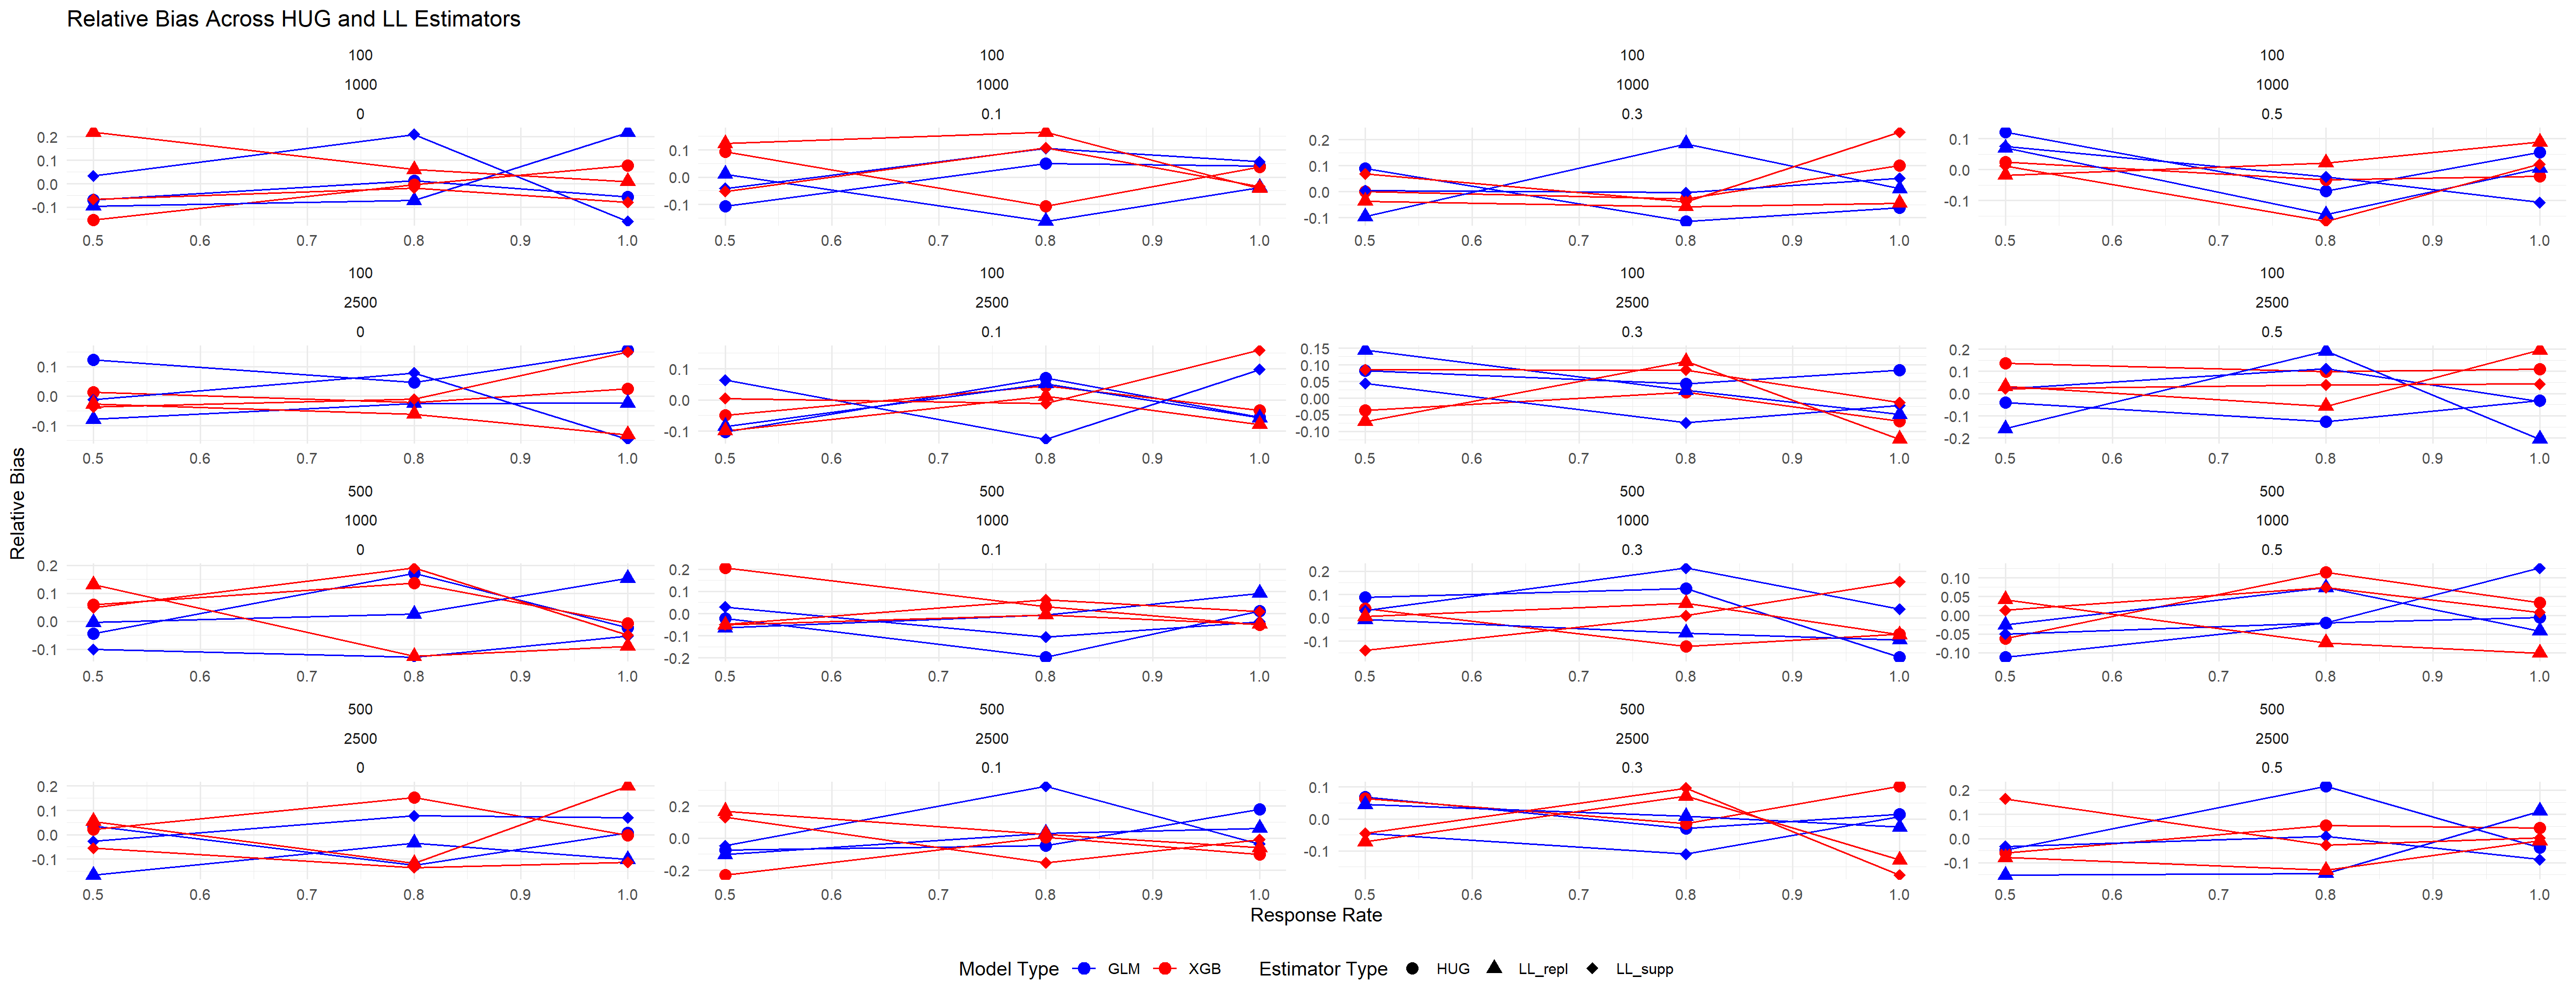
\includegraphics[width=1.8\textwidth]{Rplot02.png}  % Adjust the image file name
    \label{fig:Rplot02}
    \raggedright
    \textbf{Note.} This is simulated data and does not correspond to the expected data at all. This is merely an exemplary figure showing what a possible figure for the real results could look like.
\end{figure}
\end{landscape}


\newpage
\printbibliography

\end{document}


